\documentclass{scrartcl}

\usepackage{ucs}
\usepackage[utf8x]{inputenc}
\usepackage[english]{babel}
\usepackage{graphicx}
\usepackage{amsmath}
\usepackage{amssymb}
\usepackage[ruled,linesnumbered]{algorithm2e}
\usepackage{hyperref}

\setlength\parindent{0pt}

\title{Effiziente Algorithmen \\ Zusammenfassung}
\author{Thomas Mohr}
\date{}

\begin{document}
\maketitle
\pagebreak
\tableofcontents
\pagebreak
\listofalgorithms
\pagebreak

\section{Grundlagen}

\subsection{Stable Matching}

\begin{itemize}
	\item Eingabe: Zwei gleichgroße Mengen $ M = \{ m_1,\ldots,m_n \} $ und $ W = \{ w_1,\ldots,w_n \} $, welche in diesem Beispiel Männer und Frauen darstellen.
	\item Aufgabe: Finde paarweise Zuordnung zwischen den Elementen aus $ M $ und $ W $, so dass für jeden $ m \in M $ und jede $ w \in W $, die nicht $ m $ zugeordnet ist, gilt (Stabilität):
	\begin{enumerate}
		\item $ m $ zieht ihm zugeordnete $ w' $ gegenüber $ w $ vor, oder
		\item $ w $ zieht ihr zugeordneten $ m' $ gegenüber $ m $ vor
	\end{enumerate}
	Stabilität beschreibt hierbei, dass die Paarungen tatsächlich vorteilhaft sind für einen von beiden. D.h., wenn $ (m,w) $ ein Paar ist, aber $ m $ lieber ein Paar mit $ w' $ bilden würde, bzw. $ w $ lieber ein Paar mit $ m' $ bilden würde, so wäre ihre Verbindung instabil.
	\item Beispiel: \\
	\begin{minipage}{.5\linewidth}
		\begin{align*}
		M = \{ X,Y,Z \} \\
		X: A < B < C \\
		Y: B < A < C \\
		Z: A < B < C
		\end{align*}
	\end{minipage}
	\begin{minipage}{.5\linewidth}
		\begin{align*}
		W = \{ A,B,C \} \\
		A: Y < X < Z \\
		B: X < Y < Z \\
		C: X < Y < Z
		\end{align*}
	\end{minipage}
	\begin{itemize}
		\item Zuordnung $ (X,C),(Y,B),(Z,A) $ \\
		Ist diese Zuordnung stabil? Nein! $ X $ zieht $ A $ vor und $ A $ zieht $ X $ vor.
		\item Zuordnung $ (X,A),(Y,B),(Z,C) $ \\
		Ist die Zuordnung stabil? Ja!
		\begin{enumerate}
			\item Niemand will mit $ Z $ oder $ C $ tauschen
			\item $ X $ hat Traumfrau
			\item $ Y $ hat Traumfrau
		\end{enumerate}
	\end{itemize}
\end{itemize}

\subsubsection{Propose-\&-Reject}

\begin{algorithm}[H]
	alle $ m \in M $ und alle $ w \in W $ ''frei'' \\
	\While{$ \exists m \in M : m $ ist frei und $ \exists w \in W $ der $ m $ noch keinen Antrag gemacht hat}{
		$ w \leftarrow $ erste noch ''unbeantragte'' Frau in $ m $'s Präferenzfolge \\
		\If{$ w $ ist frei}{
			$ (m,w) $ wird Paar \\
			$ m \leftarrow $ ''verlobt'' \\
			$ w \leftarrow $ ''verlobt''
		}
		\ElseIf{$ w $ zieht $ m $ ihrem aktuellen Verlobten $ m' $ vor}{
			$ (m,w) $ wird Paar \\
			$ m \leftarrow $ ''verlobt'' \\
			$ w \leftarrow $ ''verlobt'' \\
			$ m' \leftarrow $ ''frei''
		}
		\Else{$ w $ lehnt $ m $ ab}
	}
	\caption{Propose-\&-Reject}
\end{algorithm}

\begin{itemize}
	\item Propose--Reject findet immer ein \textbf{perfektes Matching}, das stabil ist, und benötigt dazu $ \leq n^2 $ \textbf{Durchläufe} der while-Schleife.
	\item Jeder Mann bekommt die bestmögliche Frau zugeordnet (''männeroptimal'').
	\item Jede Frau bekommt den schlechtestmöglichen Mann zugeordnet.
\end{itemize}

\subsubsection{5 respräsentative Probleme}
\begin{enumerate}
	\item Interval Scheduling
	\begin{itemize}
		\item Eingabe: Intervalle mit Start- \& Endzeiten
		\item Aufgabe: Finde größtmögliche Menge nichtüberlappender Intervalle
		\item Beispiel für Greedy \\
		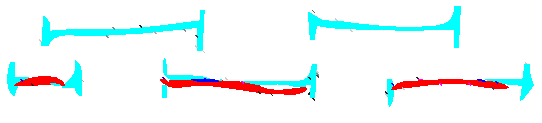
\includegraphics[width=\linewidth]{figures/interval-scheduling.pdf}
	\end{itemize}
	\item Gewichtetes Interval Scheduling
	\begin{itemize}
		\item Eingabe: Intervalle mit Start- \& Endzeiten und positiven Gewichten
		\item Aufgabe: Finde Lösung mit größtmöglichem Gesamtgewicht
		\item Beispiel für dynamisches Programmieren: \\
		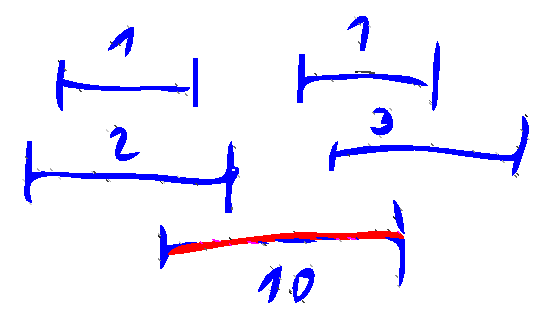
\includegraphics[width=\linewidth]{figures/gewichtetes-interval-scheduling.pdf}
	\end{itemize}
	\item Bipartites Matching
	\begin{itemize}
		\item Eingabe: Bipartiter Graph
		\item Aufgabe: Finde größtmögliche ''unabhängige'' (keine gemeinsamen Endpunkte) Kantenmenge
		\item Beispiel für Netzwerkflüsse: \\
		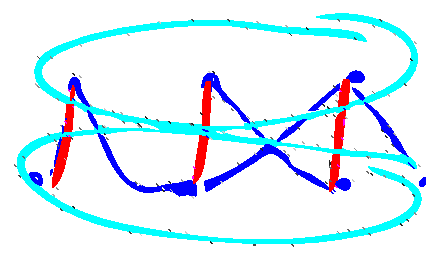
\includegraphics{figures/bipartites-matching.pdf}
	\end{itemize}
	\item Independent set
	\begin{itemize}
		\item Eingabe: Ungerichteter Graph
		\item Aufgabe: Finde größtmögliche ''unabhängige'' (paarweise nicht benachbarte) Knotenmenge
		\item Beispiel (NP-schwer): \\
		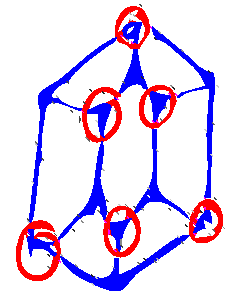
\includegraphics{figures/independent-set.pdf}
		\item Vorige Probleme sind Spezialfälle von \textbf{Independent Set}
	\end{itemize}
	\item Competitive Facility Location
	\begin{itemize}
		\item Eingabe: Knotengewichteter Graph
		\item Regeln: Zwei Spieler wählen alternierend Knoten; gewählter Knoten wird samt Nachbarn gelöscht.
		\item Ziel: Spieler 1 will Knoten so wählen, dass Spieler 2 möglichst wenige Pnkte macht
		\item Beispiel (PSPACE-vollständig): \\
		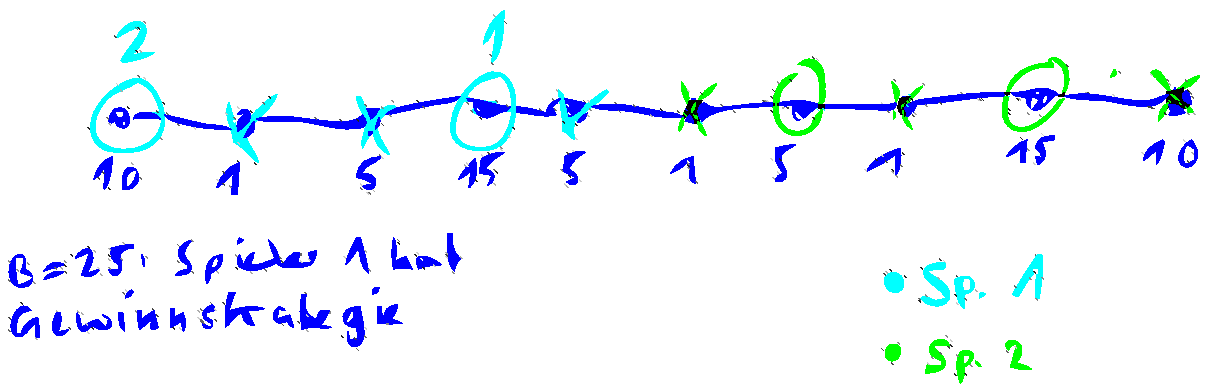
\includegraphics[width=\linewidth]{figures/competitive-facility-location.pdf}
	\end{itemize}
\end{enumerate}

\subsection{Zentrale Konzepte \& Konventionen}

\begin{itemize}
	\item Ziel \textbf{effizienter} Algorithmen: \textbf{polynomielle Laufzeit}, d.h. es existieren Konstanten $ c,d $, so dass der Algorithmus bei Eingabegröße $ n $ nach $ c \cdot n^d $ Schritten terminiert.
	\item Man beachte: \textbf{Worst-Case Analyse}
\end{itemize}

\subsubsection{$ \mathcal{O} $-Notation}

\begin{itemize}
	\item $ T(n) = \mathcal{O}(f(n)) $ falls $ \exists c > 0, n_0 \geq 0: \forall n \geq n_0 : T(n) \leq c \cdot f(n) $ \\
	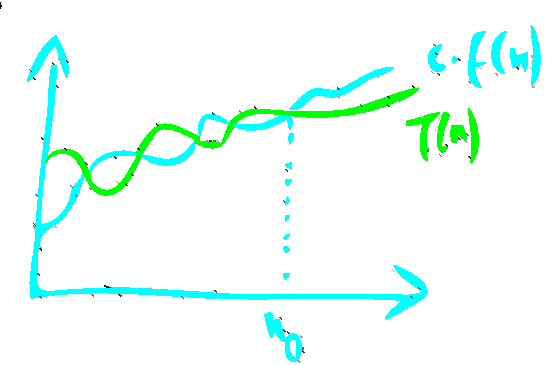
\includegraphics[width=\linewidth]{figures/o-notation.pdf}
	\item $ T(n) = \Omega(f(n)) $ falls $ \exists c > 0, n_0 \geq 0 : \forall n \geq n_0: T(n) \geq c \cdot f(n) $
	\item $ T(n) = \Theta(f(n)) $ falls $ T(n) = \mathcal{O}(f(n)) $ und $ T(n) = \Omega(f(n)) $ \\
	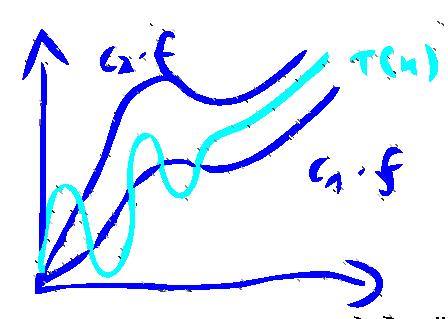
\includegraphics[width=\linewidth]{figures/theta.pdf}
	\item $ T(n) = o(f(n)) $ falls $ \forall c > 0 : \exists n_0 \geq 0 \forall n \geq n_0 : T(n) < c \cdot f(n) $
	\item $ T(n) = \omega(f(n)) $ falls $ f(n) = o(T(n)) $
\end{itemize}

Wenn die Eingabe $ n $ groß genug wird wächst $ T $
\begin{itemize}
	\item $ T(n) = \mathcal{O}(f(n)) $ \hfill nicht schneller
	\item $ T(n) = \Omega(f(n)) $ \hfill nicht langsamer
	\item $ T(n) = \Theta(f(n)) $ \hfill genauso schnell
	\item $ T(n) = o(f(n)) $ \hfill echt langsamer
	\item $ T(n) = \omega(f(n)) $ \hfill echt schneller
\end{itemize}
als $ f $.

\subsection{Graphen}

\begin{itemize}
	\item $ G = (V,E) $
	\item Konvention: $ n .= \mid V \mid, m:= \mid E \mid $
	\item Gerichteter Graph: $ e \in E $ mit $ e = (u,v), u, v \in V $ (geordnetes Paar) \\
	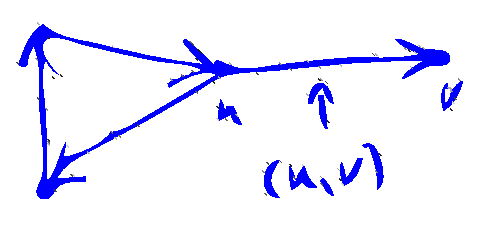
\includegraphics[width=\linewidth]{figures/gerichteter-graph.pdf}
	\item Ungerichteter Graph: $ e \in E $ mit $ e = \{ u,v \}, u, v \in V $ (ungeordnetes Paar) \\
	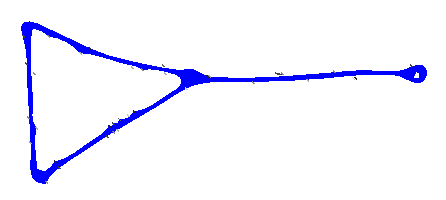
\includegraphics[width=\linewidth]{figures/ungerichteter-graph.pdf}
\end{itemize}

\subsubsection{Repräsentation}

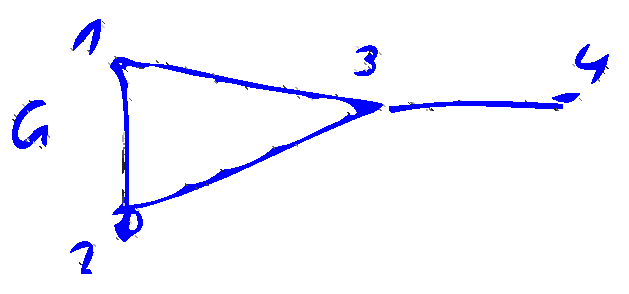
\includegraphics[width=\textwidth]{figures/graph.pdf}

\begin{itemize}
	\item Adjazenzmatrix
	\begin{itemize}
		\item $ n \times n $ 0/1-Matrix
		\item $ A_{i,j} = 1 \iff \{ v_i,v_j \} \in E $
		\item Hoher Speicherbedarf für Graphen mit wenigen Kanten (''dünn'', ''sparse'')
	\end{itemize}
	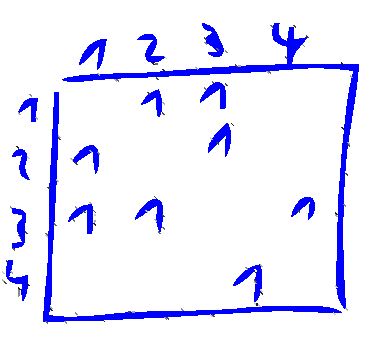
\includegraphics{figures/adjazenz-matrix.pdf}
	\item Adjazenzliste
	\begin{itemize}
		\item Array/Liste von Nachbarn für jeden Knoten
		\item Jeder Array-Eintrag führt zur Liste von Nachbarn
	\end{itemize}
	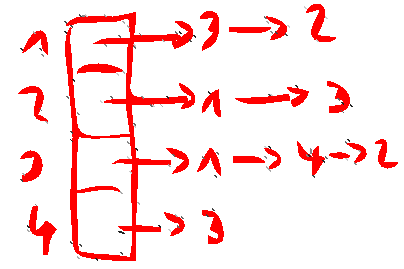
\includegraphics{figures/adjazenz-liste.pdf}
\end{itemize}

\subsubsection{Bekannte Begriffe}

\begin{itemize}
	\item Pfad: Folge von Knoten, aufeinanderfolgende sind benachbart \\
	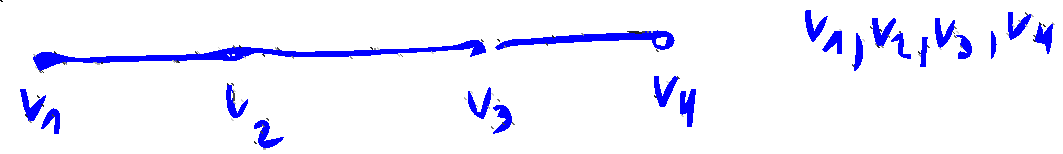
\includegraphics[width=\linewidth]{figures/pfad.pdf}
	\item Kreis: Pfad $ v_1,\ldots,v_l $ mit $ v_1=v_l $ \\
	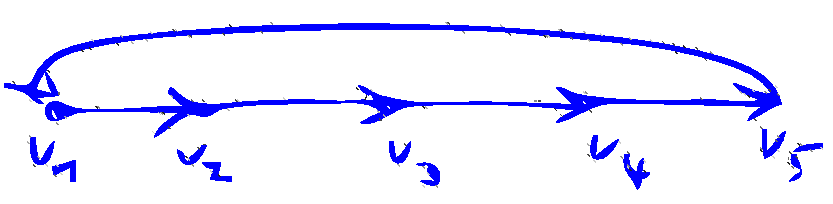
\includegraphics[width=\linewidth]{figures/kreis.pdf}
	\item Ungerichteter zusammenhängender Graph: Zwischen allen Knotenpaaren existiert ein Pfad \\
	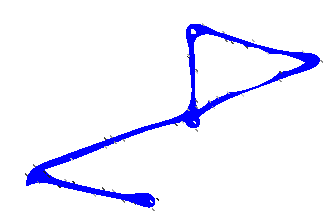
\includegraphics{figures/ungerichteter-zusammenhaengender-graph.pdf}
	\item Baum: Ungerichtet, kreisfrei, zusammenhängend \\
	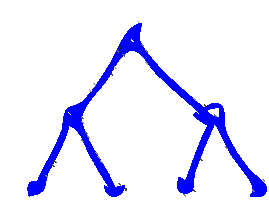
\includegraphics{figures/baum.pdf}
\end{itemize}

\subsubsection{Graphtraversierung}

\paragraph{Breitensuche (BFS)}

\begin{itemize}
	\item Idee
	\begin{itemize}
		\item Beginne am Startknoten $ s $
		\item Durchforste Graph ''schichtweise'' (erst Abstand 1 zu $ s $, dann Abstand 2, usw.)
	\end{itemize}
	\item Wichtige Datenstruktur: Schlange (FIFO)
	\item BFS kann in $ \mathcal{O}(n+m) $ Zeit durchgeführt werden
	\item Eventuell hoher Speicherbedarf
	\item Mit BFS findet man alle kürzesten Pfade ausgehend von $ s $
\end{itemize}

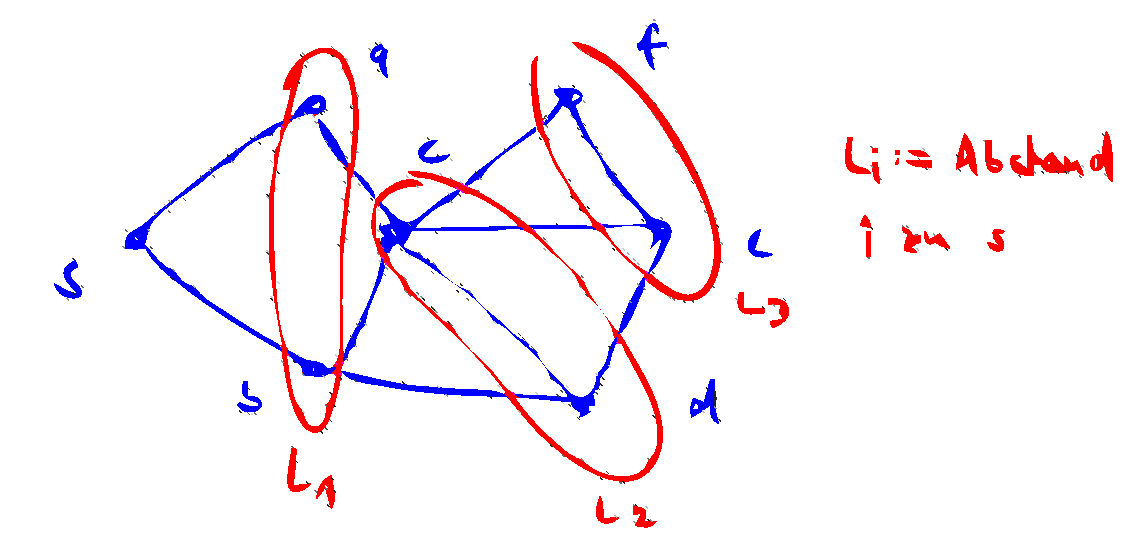
\includegraphics[width=\linewidth]{figures/bfs.pdf}

\paragraph{Tiefensuche (DFS)}\mbox{} \\
\begin{algorithm}[H]
	\KwIn{Startknoten $ u $}
	$ R \leftarrow \emptyset $ \\
	Markiere $ u $ als besucht \\
	$ R \leftarrow R \cup \{ u \} $ \\
	\ForEach{$ \{ u,v \} \in E $}{
		\If{$ v $ nicht besucht}{
			\texttt{DFS}($ v $)
		}
	}
	\KwRet{$ R $}
	\caption{DFS}
\end{algorithm}

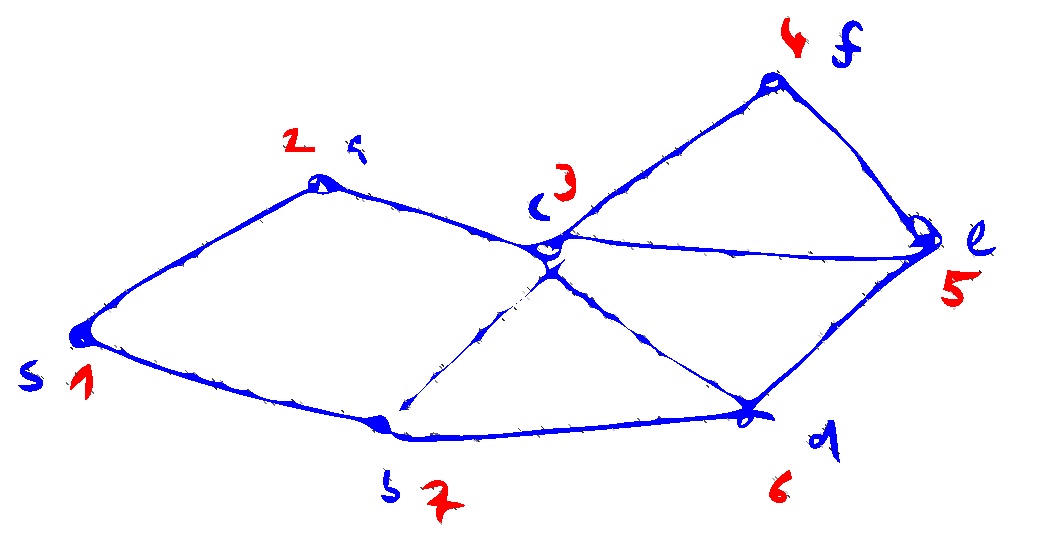
\includegraphics[width=\linewidth]{figures/dfs.pdf}

\begin{itemize}
	\item DFS kann in $ \mathcal{O}(n+m) $ Zeit durchgeführt werden.
	\item DFS findet in der Regel keine kürzesten Wege.
	\item Anwendung z.B. beim Finden von Zusammenhangskomponenten.
\end{itemize}

\subsection{Bipartite Graphen}

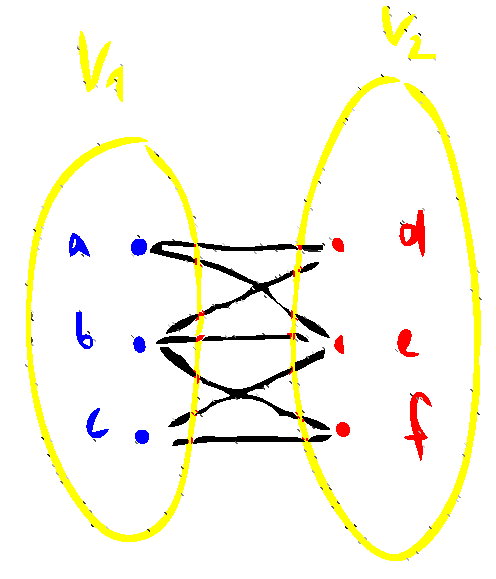
\includegraphics{figures/bipartiter-graph.pdf}

\begin{itemize}
	\item Ein Graph $ G = (V,E) $ ist \textbf{bipartit}, falls $ V = V_1 \cup V_2 $ mit $ V_1 \cap V_2 = \emptyset $ und $ E \subseteq V_1 \times V_2 $.
	\item Äquivalent:
	\begin{itemize}
		\item $ G $ ist zweifärbbar \\
		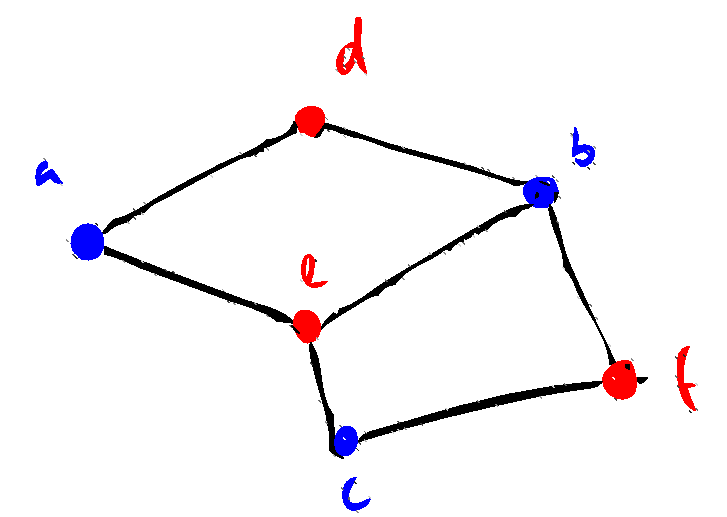
\includegraphics{figures/zweifaerbbar.pdf}
		\item $ G $ hat keinen Kreis ungerader Länge \\
		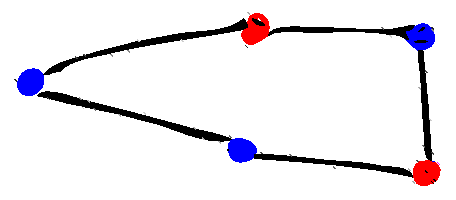
\includegraphics[width=\linewidth]{figures/kreis-ungerader-laenge.pdf}
	\end{itemize}
\end{itemize}

\subsubsection{Starker Zusammenhang}

\begin{itemize}
	\item Ein gerichteter Graph heißt \textbf{stark zusammenhängend}, falls jedes Knotenpaar \textbf{wechselseitig} durch jeweils mind. einen gerichtetetn Pfad verbunden ist.
	\item Es kann in $ \mathcal{O}(n+m) $ Zeit festgestellt werden, ob ein Graph $ G = (V,E) $ stark zusammenhängend ist.
	\item Beispiel
	\begin{itemize}
		\item Stark zusammenhängend \\
		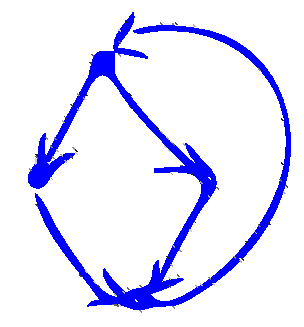
\includegraphics{figures/stark-zusammenhaengend.pdf}
		\item Nicht stark zusammenhängend \\
		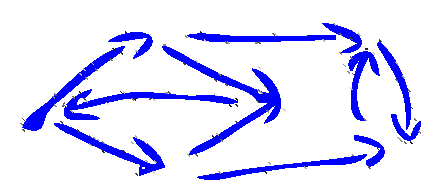
\includegraphics[width=\linewidth]{figures/nicht-stark-zusammenhaengend.pdf}
	\end{itemize}
\end{itemize}

\subsubsection{DAG's \& topologische Sortierungen}

\begin{itemize}
	\item Sei $ G = (V,E) $ ein gerichteter Graph. Eine \textbf{topologische Sortierung} ist eine totale Ordnung $ v_1,v_2,\ldots,v_n $ mit Knoten aus $ V $, so dass für jede Kante $ (v_i,v_j) \in E $ gilt: $ i < j $.
	\item DAG: ''directed acyclic graph'': gerichteter, azyklische Graph
	\item Beispiel: \\
	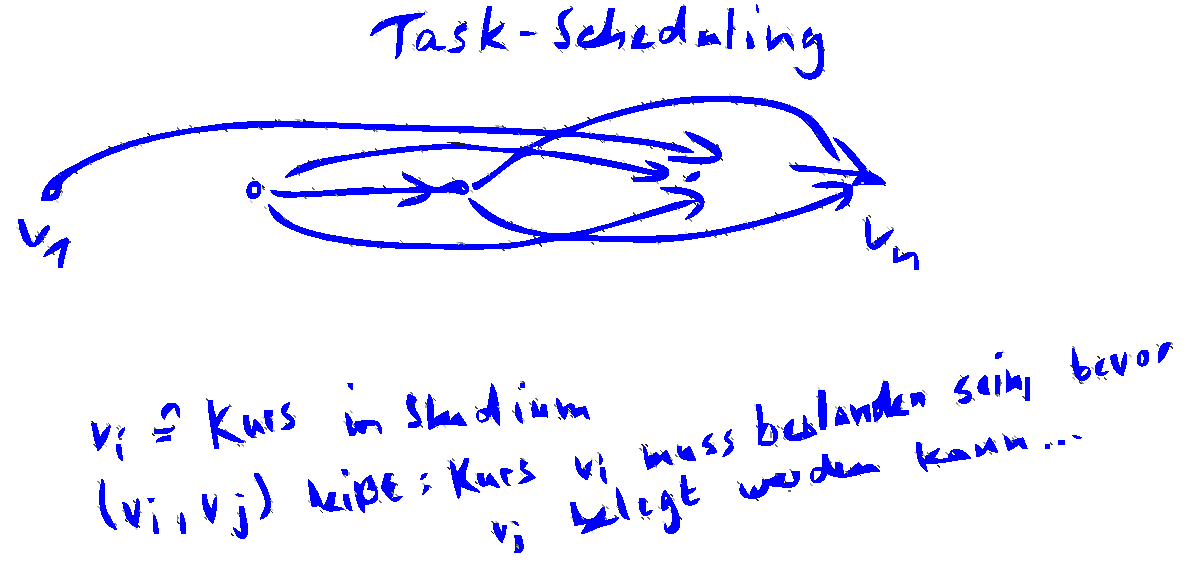
\includegraphics[width=\linewidth]{figures/task-scheduling.pdf}
	\item $ G $ ist gerichtet azyklisch $ \iff G $ hat top. Sortierung
	\item Eine topologische Sortierung eines Graphen $ G $, falls existierend, kann in $ \mathcal{O}(n+m) $ Zeit gefunden werden. Beweisidee:
	\begin{enumerate}
		\item Finde $ v \in V $ ohne Eingangskante
		\item Setze $ v $ an Spitze der Sortierung
		\item Lösche $ v $
		\item Finde Sortierung von ''$ G - v $'' rekursiv und setze diese hinter $ v $
	\end{enumerate}
\end{itemize}

\section{Greedyalgorithmen}

\subsection{Interval scheduling}

\begin{itemize}
	\item Eingabe: Intervalle (Jobs) mit Startzeiten $ s_i $ und Endzeiten $ f_i $, $ 1 \leq i \leq n $.
	\item Aufgabe: Finde größtmögliche Menge nichtüberlappender Intervalle.
	\item Greedy-Strategie: Nimm Job mit frühestmöglicher Endzeit
	\item Dieser Algorithmus liefert immer eine optimale Lösung mit Laufzeit $ \mathcal{O}(n \log n) $.
\end{itemize}

\subsection{Interval Partitioning}

\begin{itemize}
	\item Eingabe: Intervalle (Jobs) mit Startzeiten $ s_i $ und Endzeiten $ f_i $, $ 1 \leq i \leq n $.
	\item Aufgabe: Finde kleinstmögliche Menge von ''Zeitstrahlen'', so dass alle Jobs, auf diese verteilt, nicht überlappen.
	\item Die \textbf{Tiefe} einer Intervallmenge ist die maximale Zahl überlappender Intervalle.
	\item Greedy-IP liefert immer eine optimale Lösung mit Laufzeit $ \mathcal{O}(n \log n) $.
\end{itemize}

\begin{algorithm}[H]
	Sortiere Jobs nach aufsteigenden Startzeiten, d.h. $ s_1 \leq s_2 \leq \ldots \leq s_n $ \\
	$ d \leftarrow 0 $ \\
	\For{$ r \gets 1 $ \KwTo $ n $}{
		\If{Job $ j_r $ ''passt auf Zeitstrahl'' $ k \in \{ 1,\ldots,d \} $}{
			Job $ j_r $ wird Zeitstrahl $ k $ zugeordnet
		}
		\Else{
			öffne neuen Zeitstrahl $ d+1 $ \\
			ordne Job $ j_r $ Zeitstrahl $ d+1 $ zu \\
			$ d \leftarrow d+1 $
		}
	}
	\caption{Interval Partitioning}
\end{algorithm}

\subsection{Verspätungsminimierung}

\begin{itemize}
	\item Eingabe: Jobs $ j, 1 \leq j \leq n $, mit Zeitdauer $ t_j $ und ''Frist'' $ d_j $.
	\item Aufgabe: Finde Ausführungsreihenfolge der Jobs, so dass \textbf{maximale Verspätung} minimiert wird, d.h. minimiere $ L := \max_j l_j $, wobei $ l_j := \max \{ 0, f_j - d_j \} $, und $ f_j $ die Beendigungszeit von $ j $ in dieser Ausführungsreihenfolge ist.
	\item Greedy-Strategie: Führe Jobs gemäß steigender Frist $ d_j $ aus.
	\item Der Algorithmus liefert immer eine optimale Lösung mit Laufzeit $ \mathcal{O}(n \log n) $.
\end{itemize}

\subsection{Kürzeste Wege in Graphen}

\begin{itemize}
	\item Eingabe: Gerichteter Graph $ G = (V,E) $ mit Längeangaben $ l_e \geq 0 $ für jede Kante $ e \in E $, Startknoten $ s $ und Zielknoten $ t $.
	\item Aufgabe: Finde kürzesten Pfad (Summe der Kantenlängen) von $ s $ nach $ t $.
	\item Greedy-Ansatz
	\begin{itemize}
		\item Starte mit $ S := \{ s \} $.
		\item Vergrößere $ S $ schrittweise um je einen Knoten.
		\item Für jeden Knoten in $ S $ ist kürzester Pfad entdeckt.
		\item Kandidaten für Hinzunahme zu $ S $ sind Knote mit mindestens einem Nachbarn in $ S $. Erweiterung von $ S $ immer von Knoten aus, der geringste Distanz zu $ s $ hat (unter den noch nicht betrachteten Knoten).
	\end{itemize}
	\item Mittels des Algorithmus von Dijkstra lassen sich alle kürzesten Pfade ausgehend von $ s $ in $ \mathcal{O}(m \log n) $ Schritten mittels eines Priority Queue berechnen.
\end{itemize}

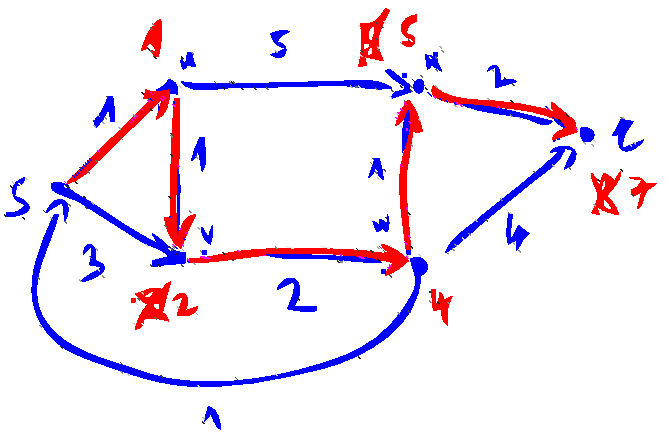
\includegraphics[width=\textwidth]{figures/kuerzeste-wege.pdf}

\subsection{Minimale Spannbäume}

\begin{itemize}
	\item Eingabe: Zusammenhängender ungerichteter Graph $ G $ mit beliebigen Kantengewichten.
	\item Aufgabe: Finde einen Baum in $ G $, der alle Knoten von $ G $ enthält und bei dem die Summe der Kantengewichte minimal ist.
	\item Berühmte Greedy-Algorithmen:
	\begin{itemize}
		\item Kruskal: Wähle ''billigste'' Kante, die keinen Kreis erzeugt.
		\item Prim: Erzeuge Baum ausgehend von einem Startknoten durch Erweiterung um billigste Kante.
	\end{itemize}
	\item Beide genannten Algorithmen können das MST-Problem in $ \mathcal{O}(m \log n) $ Schritten lösen.
\end{itemize}

\subsection{Kodierung}

\begin{itemize}
	\item Eingabe: Zeichenkette $ T $ über endlichem Alphabet $ \Sigma = \{ c_1,\ldots,c_n \} $, für jeden Buchstaben $ c_i $ eine ''relative Häufigkeit'' $ f(c_i) \geq 0 $, wobei $ \sum_{1}^{n} f(c_i) = 1 $.
	\item Aufgabe: Kodiere $ T $ über Binäralphabet $ \{ 0,1 \} $, sodass der entstehende Code minimale Länge hat.
	\item Eine Kodierung $ \gamma: \Sigma \rightarrow \{ 0,1 \}^+ $ heißt \textbf{Präfix-Code} bzw. \textbf{präfixfrei}, falls es keine zwei Buchstaben $ a,b \in \Sigma $ gibt, so dass $ \gamma(a) $ ein Präfix von $ \gamma(b) $ ist.
\end{itemize}

\subsubsection{Problemformulierung}

\begin{itemize}
	\item \textbf{Modifizierte Aufgabenstellung}: Finde eine präfixfreie Kodierung $ rightsquigarrow $ Finde vollständigen Binärbaum, dessen Blätter mit de Elementen aus $ \Sigma $ beschriftet sind (1:1), so dass die Kosten des Baums $ T $
	\[ cost(T) = \sum_{i=1}^{n} f(c_i) \cdot (\text{''Tiefe von $ c_i $ im Baum''}) \]
	minimal sind.
\end{itemize}

\subsubsection{Huffmann-Algorithmus}

\begin{algorithm}[H]
	\If{$ \mid \Sigma \mid = 2 $}{
		kodiere einen Buchstaben mit 0, den anderen mit 1
	}
	\Else{
		$ a,b := $ ''Buchstaben mit kleinster Häufigkeit'' \\
		lösche $ a $ und $ b $ aus $ \Sigma $ und füge neuen Buchstaben $ \overline{ab} $ hinzu \\
		$ f(\overline{ab}) := f(a) + f(b) $ \\
		Konstruiere rekursiv präfixfreien Code mit Baum $ T' $ \\
		Ersetze in $ T' $ das Blatt $ \overline{ab} $ durch den Unterbaum
	}
	\caption{Huffmann-Algorithmus}
\end{algorithm}

Der Algorithmus von Huffman findet in $ \mathcal{O}(n \log n) $ Zeit eine optimale präfixfreie Kodierung.

\section{Divide-\&-Conquer}

\subsection{Grundprinzip}

\begin{itemize}
	\item Zerlege Problem in mehrere (meist zwei) Teilprobleme.
	\item Löse jeden Teil rekursiv.
	\item Kombiniere die Lösungen der Teilprobleme zu Gesamtlösung.
\end{itemize}

\subsection{Rekursionsungleichungen}

\[ T(n) = aT(\lceil \frac{n}{b} \rceil) + \mathcal{O}(n^d) \]

\subsubsection{Master Theorem}

\begin{itemize}
	\item Sei $ T(n) = aT(\lceil \frac{n}{b} \rceil) + \mathcal{O}(n^d)  $ für Konstanten $ a > 0, b > 1 $ und $ d \geq 0 $, dann
	\[ T(n) = \begin{cases}
		\mathcal{O}(n^d) & \text{, falls } d > \log_b a \\
		\mathcal{O}(n^d \log n) & \text{, falls } d = \log_b a \\
		\mathcal{O}(n^{\log_b a}) & \text{, falls } d < \log_b a
	\end{cases} \]
\end{itemize}

\subsubsection{Zählen von Inversionen}

\begin{itemize}
	\item Eingabe: Eine feste Odnung $ a_1,a_2,\ldots,a_n $ der Zahlen von 1 bis $ n $.
	\item Aufgabe: Bestimme die Anzahl von Inversionen im Vergleich zur Ordnung $ 1,2,\ldots,n $, wobei eine \textbf{Inversion} ein Paar $ (i,j), 1 \leq i < j \leq n $, mit $ a_i > a_j $ ist.
	\item Lösungsansatz:
	\begin{enumerate}
		\item Teile Eingabe in 2 Hälften
		\item Zähle Inversionen je Hälfte
		\item Gesamtzahl der Invesionen = Addition de beiden Werte plus ''Inversionen zwischen den Hälften''.
	\end{enumerate}
	\item Die Zahl der Inversionen einer Folge von $ n $ verschiedenen Zahlen aus $ \{ 1,\ldots,n \} $ lässt sich in $ \mathcal{O}(n \log n) $ ermitteln. (Brute-force-Ansatz bräuchte $ \mathcal{O}(n^2) $ Zeit).
\end{itemize}

\subsection{Closest Pair}

\begin{itemize}
	\item Eingabe: $ n $ Punkte in der Euklidischen Ebene.
	\item Aufgabe: Finde Punktepaar mit geringstem Abstand.
	\item Beispiel ($ \mathcal{O}(n^2) $): \\
	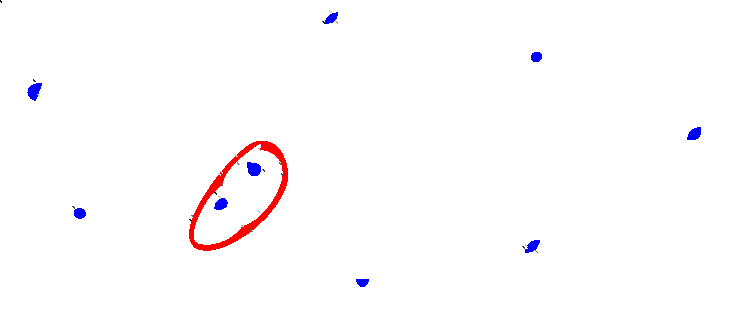
\includegraphics[width=\linewidth]{figures/closest-pair.pdf}
	\item Einfacher Spezialfall: Alle Punkte auf einer Geraden sortieren ($ \mathcal{O}(n \log n) $) \\
	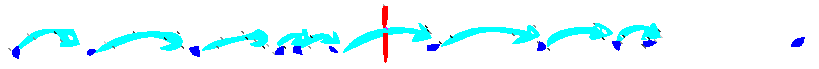
\includegraphics[width=\linewidth]{figures/closest-pair-gerade.pdf}
\end{itemize}

\subsubsection{Algorithmus}

\begin{itemize}
	\item Teile ''Punktwolke'' in zwei gleich große Hälften
	\item Paar ist entweder in einer der beiden Hälften, oder je ein Punkt in einer der beiden Hälften.
	\item Nur schmaler grenzstreifen ist zu untersuchen
	\item Jeder Punkt im Grenzstreifen ist nur mit konstant vielen anderen innerhalb des Grenzstreifens zu vergleichen.
	\item Closest Pair lässt sich in $ \mathcal{O}(n \log n) $ Zeit lösen.
\end{itemize}

\subsection{Matrixmultiplikation}

\begin{itemize}
	\item Eingabe: Zwei $ n \times n $ Matrizen $ A $ und $ B $
	\item Aufgabe: Berechne $ C = A \cdot B $
	\item Schulmethode: ''Zeile mal Spalte'' $ \rightsquigarrow \mathcal{O}(n^3) $ Elementaroperationen
	\item D\&C-Idee: Partitionierung in vier quadratische Teilmatrizen
\end{itemize}

\end{document}